\documentclass[12pt]{report}
\usepackage[spanish]{babel}
\usepackage[utf8]{inputenc}
\usepackage{amsmath}
\usepackage{amssymb}
\usepackage{amsthm}
\usepackage{graphics}
\usepackage{subfigure}
\usepackage{lipsum}
\usepackage{array}
\usepackage{multicol}
\usepackage{enumerate}
\usepackage[framemethod=TikZ]{mdframed}
\usepackage[a4paper, margin = 1.5cm]{geometry}
\usepackage{tikz}
\usepackage{pgffor}
\usepackage{ifthen}
\usepackage{listings}
\usepackage{hyperref}
\usepackage{xcolor}
\usepackage{enumitem}
\usepackage{mathdots}

%Gestión de Hipervínculos

\hypersetup{
    colorlinks=true,
    linkcolor=black,
    filecolor=magenta,      
    urlcolor=cyan
}

%Gestión de Código de Programación

\definecolor{listing-background}{HTML}{F7F7F7}
\definecolor{listing-rule}{HTML}{B3B2B3}
\definecolor{listing-numbers}{HTML}{B3B2B3}
\definecolor{listing-text-color}{HTML}{000000}
\definecolor{listing-keyword}{HTML}{435489}
\definecolor{listing-keyword-2}{HTML}{1284CA} % additional keywords
\definecolor{listing-keyword-3}{HTML}{9137CB} % additional keywords
\definecolor{listing-identifier}{HTML}{435489}
\definecolor{listing-string}{HTML}{00999A}
\definecolor{listing-comment}{HTML}{8E8E8E}

\lstdefinestyle{myStyle}{
    language         = java,
    alsolanguage     = scala,
    numbers          = left,
    xleftmargin      = 2.7em,
    framexleftmargin = 2.5em,
    backgroundcolor  = \color{gray!15},
    basicstyle       = \color{listing-text-color}\linespread{1.0}\ttfamily,
    breaklines       = true,
    frameshape       = {RYR}{Y}{Y}{RYR},
    rulecolor        = \color{black},
    tabsize          = 2,
    numberstyle      = \color{listing-numbers}\linespread{1.0}\small\ttfamily,
    aboveskip        = 1.0em,
    belowskip        = 0.1em,
    abovecaptionskip = 0em,
    belowcaptionskip = 1.0em,
    keywordstyle     = {\color{listing-keyword}\bfseries},
    keywordstyle     = {[2]\color{listing-keyword-2}\bfseries},
    keywordstyle     = {[3]\color{listing-keyword-3}\bfseries\itshape},
    sensitive        = true,
    identifierstyle  = \color{listing-identifier},
    commentstyle     = \color{listing-comment},
    stringstyle      = \color{listing-string},
    showstringspaces = false,
}

\lstset{style = myStyle}

%Gestión de Marca de Agua

\newcounter{it}
\newcommand*\watermarktext[1]{\begin{tabular}{c}
    \setcounter{it}{1}%
    \whiledo{\theit<100}{%
    \foreach \col in {0,...,15}{#1\ \ } \\ \\ \\
    \stepcounter{it}%
    }
    \end{tabular}
    }

\AddToHook{shipout/foreground}{
    \begin{tikzpicture}[remember picture,overlay, every text node part/.style={align=center}]
        \node[rectangle,black,rotate=30,scale=2,opacity=0.04] at (current page.center) {\watermarktext{Cristo Daniel Alvarado ESFM\quad}};
  \end{tikzpicture}
}

%En esta parte se hacen redefiniciones de algunos comandos para que resulte agradable el verlos%

\renewcommand{\theenumii}{\roman{enumii}}

\def\proof{\paragraph{Demostración:\\}}
\def\endproof{\hfill$\blacksquare$}

\def\sol{\paragraph{Solución:\\}}
\def\endsol{\hfill$\square$}

%En esta parte se definen los comandos a usar dentro del documento para enlistar%

\newtheoremstyle{largebreak}
  {}% use the default space above
  {}% use the default space below
  {\normalfont}% body font
  {}% indent (0pt)
  {\bfseries}% header font
  {}% punctuation
  {\newline}% break after header
  {}% header spec

\theoremstyle{largebreak}

\newmdtheoremenv[
    leftmargin=0em,
    rightmargin=0em,
    innertopmargin=-2pt,
    innerbottommargin=8pt,
    hidealllines = true,
    roundcorner = 5pt,
    backgroundcolor = gray!60!red!30
]{exa}{Ejemplo}[section]

\newmdtheoremenv[
    leftmargin=0em,
    rightmargin=0em,
    innertopmargin=-2pt,
    innerbottommargin=8pt,
    hidealllines = true,
    roundcorner = 5pt,
    backgroundcolor = gray!50!blue!30
]{obs}{Observación}[section]

\newmdtheoremenv[
    leftmargin=0em,
    rightmargin=0em,
    innertopmargin=-2pt,
    innerbottommargin=8pt,
    rightline = false,
    leftline = false
]{theor}{Teorema}[section]

\newmdtheoremenv[
    leftmargin=0em,
    rightmargin=0em,
    innertopmargin=-2pt,
    innerbottommargin=8pt,
    rightline = false,
    leftline = false
]{propo}{Proposición}[section]

\newmdtheoremenv[
    leftmargin=0em,
    rightmargin=0em,
    innertopmargin=-2pt,
    innerbottommargin=8pt,
    rightline = false,
    leftline = false
]{cor}{Corolario}[section]

\newmdtheoremenv[
    leftmargin=0em,
    rightmargin=0em,
    innertopmargin=-2pt,
    innerbottommargin=8pt,
    rightline = false,
    leftline = false
]{lema}{Lema}[section]

\newmdtheoremenv[
    leftmargin=0em,
    rightmargin=0em,
    innertopmargin=-2pt,
    innerbottommargin=8pt,
    roundcorner=5pt,
    backgroundcolor = gray!30,
    hidealllines = true
]{mydef}{Definición}[section]

\newmdtheoremenv[
    leftmargin=0em,
    rightmargin=0em,
    innertopmargin=-2pt,
    innerbottommargin=8pt,
    roundcorner=5pt
]{excer}{Ejercicio}[section]

%En esta parte se colocan comandos que definen la forma en la que se van a escribir ciertas funciones%

\newcommand\abs[1]{\ensuremath{\left|#1\right|}}
\newcommand\divides{\ensuremath{\bigm|}}
\newcommand\cf[3]{\ensuremath{#1:#2\rightarrow#3}}
\newcommand\natint[1]{\ensuremath{\left[\!\left[ #1\right]\!\right]}}
\newcommand{\afa}{\:
    \begin{tikzpicture}
        \draw [line width = 0.17 mm, black] (0,0) -- (-0.115,0.29);
        \draw [line width = 0.17 mm, black] (0,0) -- (0.115,0.29);
        \draw [line width = 0.17 mm, black] (-0.12,0) arc (190:-10:0.12cm);
    \end{tikzpicture}
    \:
}
%Este símvolo es para casi todo salvo una cantidad finita

%recuerda usar \clearpage para hacer un salto de página

\newcounter{figcount}
\setcounter{figcount}{1}

\begin{document}
    \setlength{\parskip}{5pt} % Añade 5 puntos de espacio entre párrafos
    \setlength{\parindent}{12pt} % Pone la sangría como me gusta
    \title{Notas Taller Topología Algebraica}
    \author{Cristo Daniel Alvarado}
    \maketitle

    \tableofcontents %Con este comando se genera el índice general del libro%

    %\setcounter{chapter}{3} %En esta parte lo que se hace es cambiar la enumeración del capítulo%
    
    \chapter{El Teorema de Seifert Van Kampen. Aplicaciones}
    
    \section{Introducción}
    
    Hasta ahora, hemos determinado la estructura del grupo fundamnetal de muy pocos espacios. Para aplicar el grupo fundamental en más variedad de problemas, es necesario obtener métodos para determinar la estructura de más espacios.

    Haremos una pequeña enunciación del problema a tratar: Suponga que queremos determinar el grupo fundamental de un espacio $X$ (espacio arco-conexo). Siendo
    \begin{equation*}
        X=U\cup V
    \end{equation*}
    con $U,V$ dos subespacios de $X$ que son arco-conexos. Eligiendo un punto base $x_0\in U\cap V$, uno espera que haya alguna relación entre los grupos
    \begin{equation*}
        \pi(U,x_0)\quad\textup{y}\quad\pi(V,x_0)
    \end{equation*}
    misma que nos permita decir algo sobre $\pi(X,x_0)$. Nuestro objetivo será intentar determinar y decir algo sobre $\pi(X,x_0)$ bajo estas condiciones.

    \section{Declaración y Prueba del Teorema}

    Primero, estableceremos el problema. Suponga que $U$ y $V$ son subconjuntos arco-conexos abiertos de $X$ tales que $X=U\cup V$, y que $U\cap V$ es arco-conexo no vacío. Eliga un punto base $x_0\in U\cap V$ para todos los grupos a considerar.

    \begin{theor}[\textbf{Teorema de Seifert Van Kampen}]
        Sea $H$ cualquier grupo y $\rho_1,\rho_2,\rho_3$ tres homomorfismos cualesquiera tales que el diagrama

        \begin{minipage}{\textwidth}
            \begin{center}
                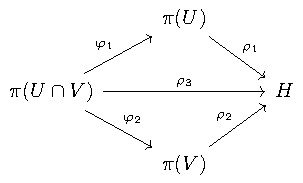
\includegraphics[scale=1.5]{images/fig_1.pdf}\\
                Figura \thefigcount. Diagrama conmutativo de los Grupos Fundamentales con $H$.
                \stepcounter{figcount}
            \end{center}
        \end{minipage}

        es conmutativo. Entonces, existe un único homomorfismo $\cf{\sigma}{\pi(X)}{H}$ tal que los siguientes tres diagramas son conmutativos:

        \begin{minipage}{\textwidth}
            \begin{center}
                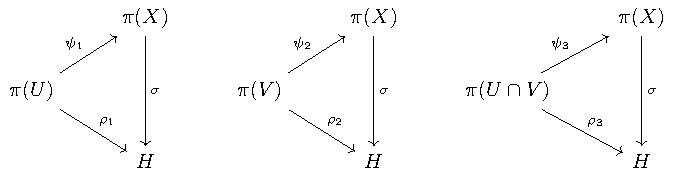
\includegraphics[scale=1.5]{images/fig_2.pdf}\\
                Figura \thefigcount. Diagramas conmutativo de $\pi(X)$ y $H$.
                \stepcounter{figcount}
            \end{center}
        \end{minipage}

        (donde los homomorfismos $\varphi_i$ y $\psi_i$ están inducidos por el mapeo inclusión, para $i=1,2,3$). Más aún, $\pi(X)$ está caracterizado hasta isomorfismos.
    \end{theor}

    Esta fue la primera versión del teorema que se probó (en su versión de dos espacios). No es nuestro objetivo actual el probar tal versión, sino una más general que involucre una cantidad arbitraria de componentes abiertas $U$ y $V$. Se verá de forma inmediata que con el siguiente teorema.

    Para ello, enunciaremos las condiciones que se requieren:

    \renewcommand{\theenumi}{\alph{enumi}}
    \begin{enumerate}[label = \textit{(\alph*)}]
        \item $X$ es un espacio arco-conexo con $x_0\in X$.
        \item  $\left\{U_\lambda \right\}_{\lambda\in\Lambda}$ es una cubierta abierta de conjuntos arco-conexos de $X$ tales que $x_0\in U_\lambda$ para todo $\lambda\in\Lambda$.
        \item Para todo $\lambda_1,\lambda_2\in\Lambda$ existe $\lambda\in\Lambda$ tal que $U_{\lambda_1}\cap U_{\lambda_2}=U_\lambda$.
    \end{enumerate}

    la condicioń (c) también se enuncia diciendo que $\left\{U_\lambda \right\}_{\lambda\in\Lambda}$ es \textbf{cerrada bajo intersecciones finitas}.

    Consideraremos los grupos fundamnetales con punto base $x_0$.

    \begin{itemize}
        \item[(*)] Si $U_\lambda\subseteq U_\mu$, entonces la función
        \begin{equation*}
            \cf{\varphi_{ \lambda\mu}}{\pi(U_\lambda)}{\pi(U_\mu)}
        \end{equation*}
        denota al homomorfismo inducido por el mapeo inclusión.
        \item[(**)] Similarmente, para todo índice $\lambda\in\Lambda$:
        \begin{equation*}
            \cf{\psi_\lambda}{\pi(U_\lambda)}{\pi(X)}
        \end{equation*}
        denota al homomorfismo inducido por el mapeo inclusión.
    \end{itemize}

    Note en particular, que si $U_\lambda\subseteq U_\mu$, entonces el diagrama

    \begin{minipage}{\textwidth}
        \begin{center}
            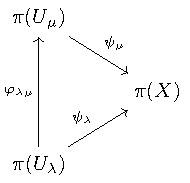
\includegraphics[scale=1.5]{images/fig_3.pdf}\\
            Figura \thefigcount. Diagramas conmutativo de $\pi(X)$, $\pi(U_\lambda)$ y $\pi(U_\mu)$.
            \stepcounter{figcount}
        \end{center}
    \end{minipage}

    es conmutativo.
    
    Ahora pasaremos con el teorema general.

    \begin{theor}
        Bajo las hipótesis anteriores, el grupo $\pi(X)$ satisface la siguiente condición de \textit{mapeo universal}: Sea $H$ cualquier grupo, y para cada $\lambda\in\Lambda$ sea $\cf{\rho_\lambda}{\pi(U_\lambda)}{H}$ un homomorfismo, tales que la familia $\left\{\rho_\lambda \right\}_{\lambda\in\Lambda}$ satisface que el siguiente diagrama

        \begin{minipage}{\textwidth}
            \begin{center}
                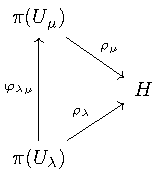
\includegraphics[scale=1.5]{images/fig_4.pdf}\\
                Figura \thefigcount. Diagramas conmutativo de $H$, $\pi(U_\lambda)$ y $\pi(U_\mu)$.
                \stepcounter{figcount}
            \end{center}
        \end{minipage}

        es conmutativo, para todo $\lambda,\mu\in\Lambda$ tales que $U_\lambda\subseteq U_\mu$. Entonces, existe un único homomorfismo $\cf{\sigma}{\pi(X)}{H}$ tal que para todo $\lambda\in\Lambda$ el siguiente diagrama

        \begin{minipage}{\textwidth}
            \begin{center}
                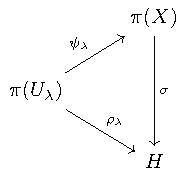
\includegraphics[scale=1.5]{images/fig_5.pdf}\\
                Figura \thefigcount. Diagramas conmutativo de $H$, $\pi(X)$ y $\pi(U_\lambda)$.
                \stepcounter{figcount}
            \end{center}
        \end{minipage}

        es conmutativo. Más aún, esta condición de mapeo universal caracteriza $\pi(X)$ hasta isomorfismos.
    \end{theor}

    Antes de hacer la prueba de este teorema, haremos la prueba de un lema que nos servirá para el teorema.

    \begin{lema}
        El grupo $\pi(X)$ es generado por la unión de las imágenes $\psi_\lambda\left(\pi(U_\lambda)\right)$, $\lambda\in\Lambda$.
    \end{lema}

    \begin{proof}
        Sea $\alpha\in\pi(X)$ y eligamos un camino $\cf{f}{I}{X}$ tal que $\alpha=[f]$. Tomemos $n\in\mathbb{N}$ tal que $\frac{1}{n}<\delta$ donde $\delta$ es el número de Lebesgue de la cubierta $\left\{f^{-1}(U_\lambda) \right\}_{\lambda\in\Lambda}$ del espacio métrico compacto $I$. Para cada $i=0,1,...,n-1$, tomemos:
        \begin{equation*}
            J_i=\left[\frac{i}{n},\frac{i+1}{n} \right]
        \end{equation*}
        Elegimos para cada $i\in\natint{0,n-1}$ un elemento $\lambda_i\in\Lambda$ tal que $f(J_i)\subseteq U_{\lambda_i}$ (el cual existe pues la medida de $J_i$ es menor que $\delta$).

        Sea ahora $f$ un camino que une a $x_0$ con $f\left(\frac{i}{n}\right)$ en $U_{\lambda_{ i-1}}\cap U_{\lambda_i}$ (el cual existe pues este último conjunto es arco-conexo y contiene a $x_0$ y al punto $f\left(\frac{i}{n}\right)$), para cada $i=1,...,n-1$. Sea ahora $\cf{f_i}{I}{X}$ el camino dado por la siguiente composición:
        \begin{equation*}
            f_i=f\big|_{J_i}\circ h_i
        \end{equation*}
        donde $\cf{h_i}{I}{J_i}$ es tal que:
        \begin{equation*}
            h_i(t)=\frac{i+t}{n}
        \end{equation*}
        así que:
        \begin{equation*}
            f_i(t)=f\left(\frac{i+t}{n}\right)
        \end{equation*}
        Entonces, los caminos:
        \begin{equation*}
            f_0\cdot g_1^{-1},g_1\cdot f_1\cdot g_2^{-1},g_2\cdot f_2\cdot g_3^{-1},...,g_{i-1}\cdot f_{i}\cdot g_{i}^{-1},...,g_{ n-2}\cdot f_{ n-2}\cdot g_{ n-1}^{-1}, g_{ n-1}\cdot f_{ n-1}
        \end{equation*}
        son todos bucles cerrados contenidos en el respectivo $U_{\lambda_i}$, con $i=0,...,n-1$. Además, el producto de todos ellos (en el orden correspondiente) es equivalente a $f$, por lo que, si hacemos:
        \begin{equation*}
            \alpha_0=[f_0\cdot g_1^{-1}],\alpha_i=[g_{i-1}\cdot f_{i}\cdot g_{i}^{-1}]\textup{ y }\alpha_{ n-1}=[g_{ n-1}\cdot f_{ n-1}]
        \end{equation*}
        para cada $i=1,...,n-2$, entonces:
        \begin{equation*}
            \alpha=\alpha_0\cdot\alpha_1\cdots\alpha_{ n-2}\cdot\alpha_{ n-1}
        \end{equation*}
        con $\alpha_i\in\psi_{\lambda_i}\left(\pi(U_{\lambda_i})\right)$, lo cual prueba el resultado.
    \end{proof}

    Ahora sí podemos pasar a la prueba del teorema.

    \begin{proof}
        Sea $H$ cualquier grupo y $\left\{\rho_\lambda \right\}_{ \lambda\in\Lambda}$ cualquier conjunto de homomorfismos que satisfaga las condiciones del teorema. Debemos mostrar la existencia de un único homomorfismo $\cf{\sigma}{\pi(X)}{H}$ tal que el diagrama:

        \begin{minipage}{\textwidth}
            \begin{center}
                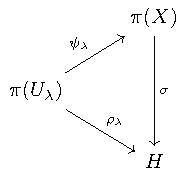
\includegraphics[scale=1.5]{images/fig_5.pdf}\\
                Figura \thefigcount. Diagramas conmutativo de $H$, $\pi(X)$ y $\pi(U_\lambda)$.
                \stepcounter{figcount}
            \end{center}
        \end{minipage}

        sea conmutativo, para todo $\lambda\in\Lambda$. Por el lema anterior, este homomorfismo (en caso de existir) es único y debe estar dado de la siguiente manera: sea $\alpha\in\pi(X)$, entonces por el lema anterior tenemos que:
        \begin{equation*}
            \alpha=\psi_{\lambda_0}(\alpha_0)\cdot\psi_{\lambda_1}(\alpha_1)\cdot...\cdot\psi_{\lambda_ {n-1}}(\alpha_{ n-1})
        \end{equation*}
        (con las respectivas observaciones del lema anterior). Por ende, si tal homomorfismo existe, debemos tener que:
        \begin{equation*}
            \sigma(\alpha)=\rho_{\lambda_0}(\alpha_0)\cdot\rho_{\lambda_1}(\alpha_1)\cdot...\cdot\rho_{\lambda_{ n-1}}(\alpha_{ n-1})
        \end{equation*}
        Para justificar esta definición, debemos mostrar que es independiente de la elección en la presentación de $\alpha$. Claramente, si es independiente de la forma de $\alpha$, entonces $\sigma$ es homomorfismo y las relaciones de conmutatividad deseadas se cumplen.

        Para probar que $\sigma$ es independiente de la representación de $\alpha$, basta con probar el lema más abajo.

        La segunda parte de este teorema no es muy complicada y es sólo un repaso de lo aprendido en grupos libres.
    \end{proof}

    \begin{lema}
        Sean $\beta_i\in U_{\lambda_i}$ como en el teorema anterior tales que $i=0,...,n-1$ tales que:
        \begin{equation*}
            \psi_{\lambda_0}(\beta_0)\cdot\psi_{\lambda_1}(\beta_1)\cdot....\cdot\psi_{\lambda_{ n-1}}(\beta_{ n-1})=1
        \end{equation*}
        entonces,
        \begin{equation*}
            \rho_{\lambda_0}(\beta_0)\cdot\rho_{\lambda_1}(\beta_1)\cdot....\cdot\rho_{\lambda_{ n-1}}(\beta_{ n-1})=1
        \end{equation*}
    \end{lema}

    \begin{proof}
        Es muy larga y tediosa pero no es díficl ya que no da nuevos métodos en la resolución de problemas. Se puede encontrar la demostración en \textit{A basic course in algebraic topology} de Massey W. S. en la página 108. 
    \end{proof}

    \section{Aplicaciones}

    Suponga como en la sentencia del teorema anterior, que $X$ es la unión de dos conjuntos $U$ y $V$, y que $U\cap V$ es arco-conexo. Sea $\varphi_i$ y $\psi_i$ tales que tengan el mismo significado que en la sección anterior.

    \begin{theor}
        Si $U\cap V$ es simplemente conexo, entonces $\pi(X)$ es el producto libre de los grupos $\pi(U)$ y $\pi(V)$ con respecto a los homomorfismos $\cf{\psi_1}{\pi(U)}{\pi(X)}$ y $\cf{\psi_2}{\pi(V)}{\pi(X)}$.
    \end{theor}

    \begin{proof}
        Sea $H$ un grupo y, $\cf{\rho_1}{\pi(U)}{H}$ y $\cf{\rho_2}{\pi(V)}{H}$ dos homomorfismos. Como $\pi(U\cap V)=\langle 1\rangle$ (en particular, es arco conexo), entonces el diagrama:

        \begin{minipage}{\textwidth}
            \begin{center}
                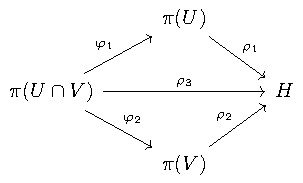
\includegraphics[scale=1.5]{images/fig_1.pdf}\\
                Figura \thefigcount. Diagrama conmutativo de los Grupos Fundamentales con $H$.
                \stepcounter{figcount}
            \end{center}
        \end{minipage}

        es conmutativo (ya que es independiente de los homomorfismos $\rho_1,\rho_2,\rho_3$ que se tomen ,más aún, el homomorfismo $\rho_3$ esta únicamente determinado). Por tanto, del teorema anterior se sigue que existe un único homomorfismo $\cf{\sigma}{\pi(X)}{H}$ tal que los diagramas:

        \begin{minipage}{\textwidth}
            \begin{center}
                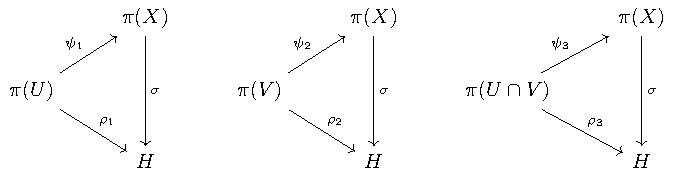
\includegraphics[scale=1.5]{images/fig_2.pdf}\\
                Figura \thefigcount. Diagramas conmutativo de $\pi(X)$ y $H$.
                \stepcounter{figcount}
            \end{center}
        \end{minipage}

        son conmutativos. En particular, el primero y el segundo diagramas son conmutativos, por lo que se tiene que $\pi(X)$ debe ser isomorfo al producto libre de los grupos $\pi(U)$ y $\pi(V)$.
    \end{proof}

    Ahora, veremos aplicaciones de este teorema.

    \begin{exa}
        Sea $X$ un espacio tal que $X=A\cup B$ y $A\cap B=\left\{x_0 \right\}$, siendo estos dos conjuntos tales que son homeomorfos al círculo $\mathbb{S}^1$. $X$ puede ser visto como la curva con forma de \textit{8}:

        \begin{minipage}{\textwidth}
            \begin{center}
                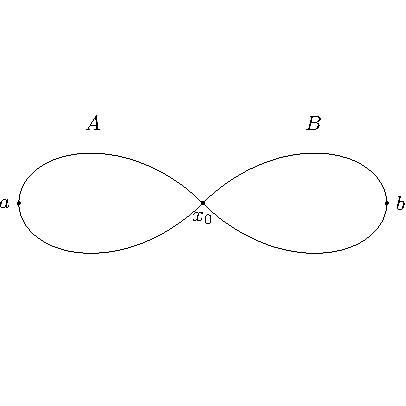
\includegraphics[scale=1.5]{images/fig_6.pdf}\\
                Figura \thefigcount. Ejemplo de la figura \textit{8}.
                \stepcounter{figcount}
            \end{center}
        \end{minipage}

        Si $A$ y $B$ fuesen subconjuntos de $X$ abiertos, podríamos aplicar de forma inmediata el teorema anterior con $U=A$ y $V=B$ para determinar la estructura de $\pi(X)$. Sin embargo, $A$ y $B$ no son abiertos.

        Pero, una pequeña modificación nos permitirá que las cosas funcionen. Elija puntos $a\in A$ y $b\in B$ tales que $a\neq x_0$ y $b\neq x_0$. Tomemos:
        \begin{equation*}
            U=X-\left\{ a\right\}\quad\textup{y}\quad V=X-\left\{b\right\}
        \end{equation*}
        entonces, $U$ y $V$ son homeomorfos a un círculo con dos \textit{colitas}. Es claro que $A$ y $B$ son deformaciones de retracción de $U$ y $V$, respectivamente. Además, el conjunto:
        \begin{equation*}
            U\cap V=X-\left\{a,b \right\}
        \end{equation*}
        es contraíble a un punto, luego simplemente conexo. Así que $\pi(X)$ es el producto libre de los grupos $\pi(U)$ y $\pi(V)$, o de forma equivalente, el producto libre de $\pi(A)$ y $\pi(B)$ (ya que $\pi(A)\cong\pi(U)$ y $\pi(B)\cong\pi(V)$). Como $A$ y $B$ son círculos, entonces $\pi(A)$ y $\pi(B)$ son grupos cíclicos infinitos. Así que $\pi(X)$ es el producto libre de dos grupos cíclicos infinitos, por una proposición anterior, $\pi(X)$ es grupo libre sobre un conjunto con dos elementos. Podemos tomar como generadores clases de caminos cerrados $\alpha$ y $\beta$ con punto base $x_0$, que van alrededor de $A$ y $B$ una vez, respectivamente.
    \end{exa}


\end{document}